% Compile with XeLaTeX or LuaLaTeX
\documentclass[10pt,a4paper]{article}



\usepackage[linesnumbered,boxed,algosection]{algorithm2e}
\usepackage{xcolor}
\usepackage{titlesec}
\usepackage{fontspec}
\defaultfontfeatures{Mapping=tex-text}
\usepackage{xunicode}
\usepackage{xltxtra}
\usepackage{polyglossia}
\usepackage{amsthm}
\usepackage{indentfirst}             % 段首缩进
\newtheorem{mydef}{Definition}
\newfontfamily\menlo{Menlo}
\setdefaultlanguage{english}
% 设置字体
\setsansfont{Consolas}
\setmainfont[BoldFont=SimHei]{STKaiti}
\usepackage{amsmath}
\usepackage{amsfonts}
\usepackage{amssymb}
\usepackage{graphicx}
% 设置页边距
%\usepackage[left=2cm,right=2cm,top=2cm,bottom=2cm]{geometry}
% MATLAB代码插入包
\usepackage{listings}
% 新定义字体
\newfontfamily\song{SimSun}          % 宋体
\newfontfamily\hei{SimHei}           % 黑体
\XeTeXlinebreaklocale "zh"           % 中文断行

% Define a new fontfamily for the subsubsection font
% Don't use \fontspec directly to change the font
\newfontfamily\subsubsectionfont[Color=MSLightBlue]{Times New Roman}
% Set formats for each heading level
\titleformat*{\section}{\Large\bfseries\sffamily\hei}
\titleformat*{\subsection}{\large\bfseries\sffamily\hei}
\titleformat*{\subsubsection}{\subsubsectionfont\hei}


\lstset
{
	language=Java,
	numbers=left,
	basicstyle=\small\menlo,
	xleftmargin=4em,
	keywordstyle=\color[RGB]{0, 0, 255},
	commentstyle=\color[RGB]{0, 128, 0},
	frame=shadowbox,
	rulesepcolor=\color{red!20!green!20!blue!20}
}
\author{胡子牛  1400012798\\[2ex]
    北京大学信息科学技术学院\\[2ex]}
\title{编译实习报告}
\date{Jan 5, 2017}
\begin{document}

%%%% 段落首行缩进两个字 %%%%
\makeatletter
\let\@afterindentfalse\@afterindenttrue
\@afterindenttrue
\makeatother
\setlength{\parindent}{2em}  %中文缩进两个汉字位

\maketitle

\section{类型检查}

\subsection{问题概述}
lab的第一部分要求对任意符合语法规则的minijava程序输入进行初步的语义分析,从而确定其是否符合一些基本的语义规则。该试验先用javaCC生成的抽象语法树解析器(AST Parser)对输入程序先构造抽象语法树,并基于此进行类型检查。

为了确定每一个语句是否符合基本的语义规则,比如变量类型是否匹配,类调用函数是否符合申明格式之类,必须了解关于变量、类在语句所处的上下文环境里的定义信息。因此在做检查之前须先构建符号表。构建好符号表之后,根据其信息和程序上下文对每一个可能的错误进行诊断。

\subsection{符号表构建}
符号表的功能是描述整个程序的逻辑结构,程序源代码中的每个标识符和他的声明、使用信息绑定在一起存储在符号表中,需要存储的内容包括数据类型、作用域和使用情况(比如转kanga的DU链)。由于这一部分里,minijava所有的声明都在函数的开始,不会在嵌套括号中声明,大大减小了符号表的维护难度。在这个情况下最小的作用单元仅为一个函数,而所有函数均归属于某一个类(不存在全局函数,即便存在可以认为属于main类)。而在每一个函数单元里我们需要记录她的变量信息,将标志符和类型进行对应记录其中。
基于以上分析,我得到了如Fig.\ref{fig:umla}的符号表整体构建思路:
\begin{figure}[ht]
\centering
  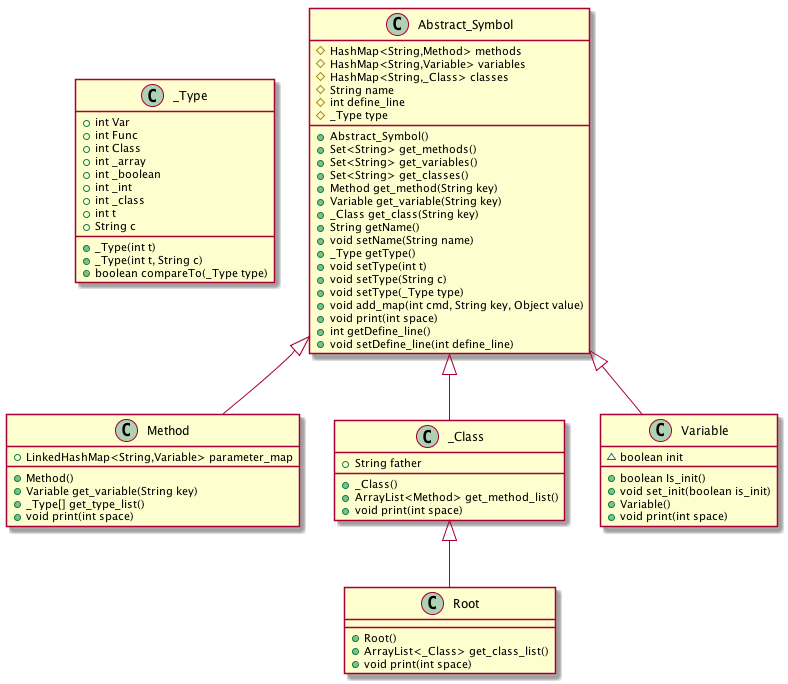
\includegraphics[width=1\textwidth]{uml1.png}
  \caption{符号表的UML图.}~\label{fig:umla}
\end{figure}

\begin{enumerate}
      \item  符号表包含三种基本类型的符号元素,分别是Method, \_Class, Variable。由于每个元素都可能具有一些包含包含关系(比如class包含成员函数和成员变量,method包含初始化定义的变量等),在设计时将它们公有的信息提取出来作为基类Abstract\_Symbol,包含关系使用hashtable来实现。 
      \item  对于Method来说,需要额外记录它的形参列表和返回值。对于\_Class来说,需要额外记录类的继承关系。由于minijava没有多继承特质,只需要记录一个父节点即可。对于Variable,可以记录一下它在程序执行过程中有没有初始化(为了判断之后有没有未define即use,粗略的筛除)
      \item  在具体执行时,所有程序均在一个函数体内。此时程序可以访问到的变量有函数体声明的局部变量、传入的参数、以及函数所在的类的成员变量。
      \item  为了方便之后进行变量类型的比较,自己实现了一个\_Type类用以记录某一个symbol的类型,并实现了compare函数方便之后比较。
\end{enumerate}
符号表建立需要一次便利整个AST,由于按照深度优先遍历,在对每个函数进行遍历的时候必然已经建立好它所在的类\_Class节点了,只需要在回溯的时候将该Method节点加入\_Class节点的函数table中即可。

\subsection{错误检查}

符号表建立完成后即可开始错误检查。讲义中要求我们找出8个错误和一个\\bonus。将其简单分类:
\begin{enumerate}
	\item 函数变量重复定义、循环继承、方法重载可以在符号表建立过程中和建立结束后直接进行检查。我称之为静态定义错误。
	\item 函数变量未定义,运算符操作数类型匹配、变量类型匹配、方法参数、返回值匹配,需要第二次对程序进行遍历,借助符号表完成。	\(bonus\)未初始化的变量不可以使用。这个也可以在第二次遍历过程中实现。我称之为动态分配错误。
\end{enumerate}
下面就对这两部分依次进行讨论实现细节。

\subsubsection{静态定义错误}

	这一部分只和程序的定义部分有关,只需要在符号表建立过程中和建立后对其进行分析即可。其中函数变量重复定义的问题只需要在建立符号表时留意在准备将一个元素加入符号表示,判断之前是不是已经加入过了。如果是,说明该变量被重复定义了。
	
	较为复杂的是关于循环继承和方法重载的问题。由于minijava允许重写但不允许重载,即子类可以有一个方法和父类的某方法方法名、变量列表、返回值完全匹配,但不允许方法名一样但变量列表或者返回值不同。因此,在获得了符号表中所有类的继承关系(每个类有一个父类引用)之后,可以利用它构建一个继承图。
	
	之后对该图进行判环。标准做法可以用拓扑排序,但因为在本例中每个节点至多只有一个父节点,只需从任意一个没有遍历过的节点开始往后不断遍历看是否会跳到之前出现过的节点即可。如果该图有环,则势必出现了循环重载;如果无环,每一个类都处在有且仅有一个继承链中(因为每个类至多继承一个父类),则只需要从链头开始记录该链的方法列表,每到下一个节点,判断该节点中的所有方法是否和当前列表中任何一个重载匹配,即类名相同,但方法、返回值不完全相同。如果没有,则加入列表中,如果有,则必然出现重载问题。
	
	至此,静态定义错误全部检查完毕。算法并不复杂,就不过多赘述了。

\subsubsection{动态分配错误}
	
	下一步进行动态分配错误的检查。动态分配错误主要是一个变量应该是某一个类型,但是在其被使用的位置被赋上了类型不匹配的值、抑或是被于类型不匹配的位置。由于这个错误是在程序使用段出现的,必须得再一次遍历AST。
	
	动态分配错误包含非常多的分项,但归根结底就是在语法树使用到规约到某一个变量的时候,其上下文约束这个位置需要出现某一个类型,但是实际上这个变量却不是这个类型。而在minijava的BNF语法中,涉及到规约到某一个变量的节点是Expression和PrimaryExpression。因此在程序中,只需要针对这两类所在的上下文判定出这个位置需要填什么类型的变量,再同其真实值的标志符对应的类型进行比较。如若不同,则出现动态分配错误。
	
	其中较为复杂的表达式是调用方法的。因为minijava允许子类调用父类的方法,在调用某函数时,需要先找到当前类所在的继承链,然后从头到尾扫描一遍找到和当前方法名一样的方法(若找不到则调用了未定义方法),之后判断参数列表和返回值是否匹配。因为前文提到不允许重载,所以只要标志符相同则一定意味着参数列表相同,减少了部分工作量。
	
	bonus要求找出未初始化即使用的变量。实际上这一步想要完美作出必须得分析程序执行流,知道跳转关系,方能较为准确的获知是否出现这个情况。在只拥有符号表的前提下,可以做保守估计,假设在整个函数体中均为定义,但有一处使用,则认为它可能错(实际上使用处可能是永远不会到达的死代码,比如if(false);	但我们没法获知这个信息,只能在出现这种情况的时候提示warning)。
	
	其他的几个表达式只需要按照要求找到对应类型即可。不再过多赘述。


\section{Minijava 转 Piglet}

\subsection{问题概述}

这一部分任务要求把minijava转成piglet中间代码。minijava是一个面向对象的,以类为核心的高级语言,要想真实运行必须最终转变成只包含基本运算和跳转的汇编指令。那么一个难点就是如何将继承、重载等面向对象的高级机制翻译成低级语言。piglet中间代码即突出了这个问题。

piglet是一种接近中间代码的语言,采用后缀表达式,操作符放在最前面,并不是严格的三地址代码。但是它取消了类的设定,整个程序是面向过程的代码。

在真实进行翻译时,原本在java里以一个封装类表现的对象,在piglet中需要显示地为他开辟一段空间,把类的成员变量和成员方法地址信息依次填入这段空间。需要开多大,如何存放,都是在翻译的时候决定好的。因此在翻译之前必须得明确地知道每一个对象内部需要存放什么信息。

处理好面向对象之后,其他就只是基本的语法制导翻译的内容了。需要注意数组的处理、过程调用的处理等。由于piglet采用的是后缀表达式,可以用类似递归调用的方式来处理一些嵌套、赋值,基本上每一个翻译都是顺序进行的,和\\minijava的语句顺序基本一致。

\subsection{处理类结构}

在面向对象语言中,类是操作的主体,变量和过程都是类的一部分。然而在piglet中数据类型只有基本类型,必须讲类拆分开,对每一个对象显示地开辟空间放入合适的内容。由于我们知道每一个对象是什么类的,只需要将这个类可以访问到的所有数据作为他的内容即可。

在minijava中,子类可以访问自己以及继承链上所有父节点的变量和方法。因此需要用到上一节中构建符号表中的继承链。将每个类可以访问到的所有变量、方法,以及相对应的她们在对象空间里的相对位置存放在一个表中。和一些同学的做法不同,我认为没有明显的必要区分变量和方法,可以把他们混杂在一起放在一个访问表里。这个表需要根据程序对某个对象的上下文状态以及调用他的成员标志符,决定最终返回该对象哪个位置的信息(是变量的位置还是方法的位置)。

\subsubsection{处理继承}

处理类结构最难的部分就是处理类之间的继承关系了。对于变量和方法,继承的行为不同。不是一般性的,考虑类A继承类B。
\begin{itemize}
	\item 假设c是A,B公有的同名变量,新变量A.c并不会把旧变量B.c的空间占去。虽然在具体程序运行的时候,类A调用c只能获取自己的那部分空间,但是如果把A强制类型转换成B,即可访问B.c的内容。因此在构建上文描述的表时,需要把继承链上所有的变量信息都保留。但在具体访问的时候只取最靠近当前类所属的变量。

	\item 假设f是A,B共有的同名函数,A.f将会覆盖B.f。这样即便讲A强制转化为B类型,调用f时也会调用A的方法。以此实现多态。因此在构建表时,当需要添加方法f时,需要遍历一下继承链上所有的para列表,保证如果发现和需要添加的方法f重名,将其覆盖。构建时从继承链的头开始依次添加覆盖,可以保证每个类的表中每个方法的名字都不重复。
\end{itemize}

\begin{lstlisting}
class Test{
	public static void main(String[] a){
		QS q = new QS();
		PS p = new PS();
		q.rush(d);		 // QS.rush
		p.rush(d);		 // PS.rush
		((QS)p).rush(d);	 // PS.rush
		((QS)p).x;		 // QS.x
		p.x			 // PS.x
	}
}

class QS{
	int x;
	public QS(){
		x = 2;
	}
	public int rush(int d){
		return d+x;
	}
}

class PS extends QS{
	int x;
	public PS(){
		x = 1;
	}
	public int rush(int d){
		return d+x;
	}
}
\end{lstlisting}

\subsubsection{实现细节}

具体实现细节如Fig.\ref{fig:umlb}的数据结构。其中para是变量、方法的抽象表示,包含一些基本信息。Dispatched\_table即前文提到的对每个类可以访问到的变量、方法的表。它是一个二位的链表。第一个维度是继承链上的类名,对每一个类,第二个维度是他所对应的所有变量、方法(para)。构建时按照前述方法,方法覆盖变量不覆盖。

具体调用变量时,从最靠近当前类的位置寻找变量,找到则返回。调用方法是,因为每个方法至多只含一个,只要找到即可返回。统一返回para对应的偏移量。

为了实现对象内的函数调用,穿参数是第一个参数预留给对象本身。如果在函数内使用本地变量,直接使用相应的寄存器存取。如果使用的是类的成员变量,以TEMP0为基地址,依据Dispatched\_table中变量相应的偏移位置,存取对应内存区域(即为对应成员变量)。其他的参数按照piglet的要求进行传递,如果有多于20个参数,则把所有参数放入TEMP1所在的地址空间处。

\begin{figure}[t!]
\centering
  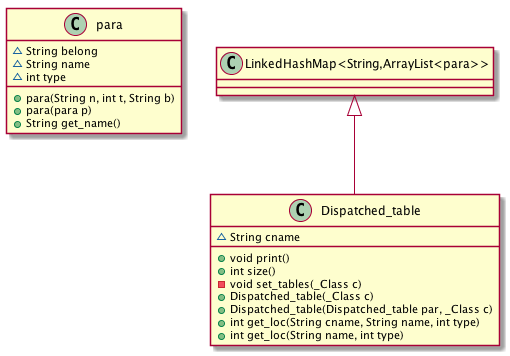
\includegraphics[width=0.75\textwidth]{uml2.png}
  \caption{minijava类结构的UML图.}~\label{fig:umlb}
\end{figure}
\subsection{处理数组}

由于piglet要求获得数组长度,并拥有预判是否因为访问数组越界而引发错误(上一个作业的bonus,在这里可以完美实现),我们给数组开辟空间的时候多开一位存储数组长度。这样一来方便获取数组长度,二来在进行数组访问的时候可以先取出长度进行预判,是否会出现数组越界。程序中代表数组的只是数组首地址。

\subsection{语法制导翻译}

将以上两部分预先处理解决好后,即可逐行对minijava进行语法制导翻译。翻译时有两件事需要注意。第一是由于在处理成员变量时需要知道当前所在的上下文信息,所以需要记录当前所在的类、函数,以及当前的Dispatched\_table。第二是由于piglet对于变量的标志是使用寄存器的,所以在翻译时还需要维护在当前函数上下文内的变量符号表。该表的目的是将minijava的标志符和变量的地址进行映射(包括寄存器和内存)。变量符号表和上下文一一绑定,因为一旦切换到另一个函数,所有寄存器将清零(piglet的做法)。不过虽然没有在程序里显示表示,但在具体执行的时候调用函数之前piglet解释器会将当前寄存器保存,返回时恢复,所以不必担心。

下面以几个较为复杂的语句翻译为例介绍一下翻译模式。

\subsubsection{超过20个参数的函数调用}

前文提到超过20个参数是可以把所有参数放到TEMP1所开辟的空间,方便所有寄存器统一处理。为了让之后赋值和取值是可以快速得到参数的位置,最好不要每次都去查Dispatched\_table计算得到。于是考虑讲变量信息存入变量符号表。为了区分存入内存的和寄存器的,我的处理方式是放入内存的位置都取负值,而放入寄存器的是正值。这样可以快速的识别并且和位置一一对应。这么做只在本次作业可行,因为唯一需要压入内存的全部存在了TEMP0和1处。未来要做必须得建立完善的数据结构。

\subsubsection{赋值、数组赋值}

赋值的难点在于准确的找到被赋值的数据位置。从minijava语句里可以得到被赋值的变量的名字,通过名字可以知道该变量是成员变量,局部变量还是函数调用的实参。根据不同的身份有不同的处理方式。
\begin{itemize}
	\item 如果是成员变量,借助传递来的TEMP0,获取到对象地址。再根据\\Dispatched\_table得到的偏移量,计算得到成员变量的内存地址,进行存取。
	\item 如果是局部变量,判断是否进行过初始化,即有没有被分配寄存器空间,并在寄存器表中有记录。如果没有,多开一个寄存器给他,加入寄存器表。寄存器分配从20开始(前20个留给函数传参使用。现阶段不做寄存器优化)。
	\item 如果是函数参数,判断该函数参数是否有超过20。如果没有则直接按序号取。如果超过了,则从栈中取。       
\end{itemize}    

数组赋值基本和普通数赋值同理,除了之前提到的数组需要判断一下这次赋值操作有没有超出数组的长度。如果超出了直接报error。

\subsubsection{逻辑运算和控制语句}

逻辑运算中较为麻烦的是与运算。因为piglet没有与运算符,所以需要利用比较和条件转移指令来实现与运算。具体细节即假设A \&\& B,若希望为真必须两个都为1,于是分别将A,B同0进行比较,如果相同跳到失败区,返回0,连续两次成功才能返回1。

拥有逻辑运算机制后,即可进行控制语句,例如if和while。并不难实现。

其他的语句也不难翻译,逐条翻译即可。

\section{Minijava 转 Spiglet}

Spiglet代码和piglet最大的区别就是删去了后缀表达式造成的复合语句。没有了StmtExp。有很多同学直接从piglet转spiglet,只需要对原来出现复合表达式的极少数情况做处理即可。但当时我没有听清题意,做成了minijava转spiglet,做法就完全不同了。。。。

minijava转spiglet最大的麻烦之处就是有更多的地方需要做回填。比如函数调用,所有的参数都得先实现算好暂存在一个列表里再放进去,诸如此类的回填特别多。最恶心的就是之前为了防止数组越界,要先判断访问下标和数组长。由于其中牵扯到一些四则运算和比较,在piglet里面都可以通过复合表达式处理成一句话,但spiglet必须讲他们每个都拆开,修改的较多。

虽然多花了不少时间,但是这一部分难度确实不高。

\section{Spiglet 转 Kanga}

\subsection{问题概述}

这一部分是整个编译器实现里难度最大的一节。

Kanga作为面向MIPS的中间代码,和Spiglet相比有一些重要的变化:
\begin{enumerate}
	\item 除极少数赋值指令外均实现了三地址代码(其实感觉完全可以一步mips的)。
	\item 引入了运行栈,调用函数时保存寄存器需要自己手动完成了。
	\item 调用函数时不再有显示调用参数,需要通过固定的寄存器和堆栈进行传参。同时没有显示的返回值。
	\item 最最主要的区别就是Kanga的语法里寄存器数量变得有限(24个)。要将spiglet中无限使用的寄存器缩减到24个,需要实现寄存器分配。
\end{enumerate}

可以说这部分最难的地方就在于寄存器分配。在之前的翻译中,寄存器基本就是有需要就开一个,但那样显然不符合实际。有大量寄存器使用一次过后再也没有使用,却依然占据着位置。合理的寄存器分配应该用尽可能少的寄存器完成一个程序任务。

而想要做到高效分配寄存器,就必须做变量的活性分析,了解在某一个时刻哪些变量活跃,需要寄存器来承接这些值;什么时候不太活跃,但未来需要被用到所以不能丢弃,于是暂存栈中;什么时候完全没有使用价值,可以被丢弃。

提到活跃性分析就可以想到在类型检查时的bonus,判断哪个变量未初始化即被使用。当时我们没有办法完整的做出判断,因为不知道程序的控制流。但现在如果要做活跃性分析,必须知道程序的执行顺序,也就是控制流。在构建好控制流的基础上,可以计算每个变量的DU链,了解在某个时刻哪些变量不能共存,建立干扰图。之后利用图染色算法即可得到一个可行的寄存器分配解。

\subsection{控制流分析}

首先我们对spiglet程序进行控制流分析,建立流图。流图是程序可能的执行跳转图,每个节点是一个基本块。基本块是程序中一个连续的语句序列,每次执行都从这个序列的第一句话开始顺序执行到最后一句话。流图示表示各基本块执行次序的有向图。

寻找基本块需要先找到它的开头,也就是入口语句。基本块有如下性质:
\begin{itemize}
	\item 过程的第一个语句是基本块的入口语句。
	\item 过程中任何由Label开始的语句都是基本块的入口语句。
	\item 任何紧跟在JUMP和CJUMP后的语句都是基本块的入口语句。       
\end{itemize}  

找到所有入口语句后,每个基本块就是任一个入口语句到下一个入口语句之前语句话之间的程序段。由此可以构建出每个基本块,且由一个入口语句连接的两个基本块在流图上被边相连接。因此,通过一次遍历即可构建出流图。

在构建的过程中我们能知道每一条语句定义或者使用了哪些变量。这些语句(Operation)是基本块的元素,而基本块是流图的元素。数据结构见Fig.ref{fig:umlc}.

\begin{figure}[t!]
\centering
  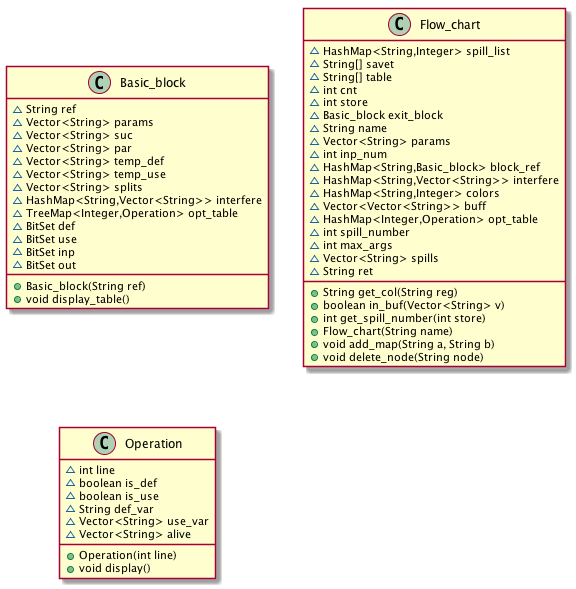
\includegraphics[width=0.8\textwidth]{uml3.png}
  \caption{控制流图的UML图.}~\label{fig:umlc}
\end{figure}

\subsection{活性分析}

进行活性分析的要点在于找出在某一时刻哪几个变量同时活跃。活跃的意思是在之后的某一时刻该变量要被使用,而在这过程中这个变量没有被赋予新值。因此这个变量在这个时刻需要被保存,也就是需要寄存器。显然,同时活跃的变量不能共享寄存器。

由于在之前的翻译过程中,我们没有重用任何寄存器,不同寄存器

构建完流图以后,我们首先以基本块为单位进行活跃性分析,解出在每个基本块的入口和出口有哪些变量还活跃。因为我们知道当知道了在一个基本块开头和结尾处活跃的变量以后,中间顺序执行非常好计算。但在流图中反复跳转不确定性很大,复杂度较高。

\subsubsection{块间分析算法}

由于之前在构建流图的时候,知道了基本块每个语句定义或者使用了哪些变量。通过简单的加和即可知道一个基本块整体上DEF了哪些变量,USE了哪些变量(注意,一个变量属于USE的前提是在这个基本块里他在被使用的语句之前没有别的语句给他赋值,属于DEF同理,被赋值之前不能有语句使用了他。)将以上原则用定义表示即:


\begin{mydef}
    一个寄存器$v$在$p$点活跃当且仅当$v$在某个以$p$开始的路径上被读取了(use)并且没有写入(def)出现在这个读取之前。同理,一个寄存器$v$在$p$点不活跃当且仅当$v$在没有一个以$p$开始的路径上被读取了(use)或者所有以$p$开始的路径上写入(def)都出现在这个读取之前。
\end{mydef}

根据这个定义,给出算法:

\begin{algorithm}
\small
    \caption{活跃性分析. }
    \SetAlgoLined
    \KwIn{$N = $basic block set , $Exit = $last node in basic blocks}
    \KwOut{$IN$, $OUT$, $USE$, $DEF$}
    \SetAlgoLined
      \ForEach{$n \in N-{Exit}$} {
          $IN[n] \leftarrow \varnothing $\\
      }
      $OUT[Exit] \leftarrow \varnothing$\\
      $IN[Exit] \leftarrow USE[Exit]$\\
      $Changed \leftarrow N - {Exit}$\\
      \While{$Changed \neq \varnothing$}
      {
      		choose a node n $ \in Changed$ \\
			$Changed \leftarrow Changed - {n}$ \\
			$OUT[n] \leftarrow \varnothing$\\
			\ForEach{$s \in successors(n)$} {
          		$OUT[n] \leftarrow OUT[n] /cup IN[s]$\\
      		}
			$IN[n] \leftarrow USE[n] /cup (OUT[n] - DEF[n]) $\\
			\If{$IN[n] changed$}
			{
				\ForEach{$p \in successors(n)$} {
          			$Changed \leftarrow Changed /cup {p}$\\
      			}
			}
	  }
    \label{tab:algorithm}
\end{algorithm}

\subsubsection{图染色}

得到基本块首尾的活跃信息以后,开始对基本块内逐条语句进行分析。原则和之前一样,遇到def即将变量移除活跃列表,遇到则加入。在某一语句上的活跃列表互相之间干扰,于是根据这个信息建立干扰图。

实际上在如何构建干扰图上我是有过挣扎的。如果说我之前转piglet的代码不是非常贪心的需要一个寄存器就放一个,而是有少量的回收,也就是可能会有寄存器跨越两个不连续的DU链,那么以变量为节点可能导致过分保守。比如在一个基本块里,只在开头a与b冲突,但之后ab先后到达use点。之后一段时间a再一次被def,此时b没有活跃,可是a却要收到b的影响染色数少1.这样是不合理的。对于这种情况,更合适的做法是用DU链为节点。如果要那么做,可以对现在的图做一次遍历,找出所有的DU链以及他们的跨度和相互干扰,以此建图。幸好我的转piglet代码是贪心策略,导致我的每一个寄存器号就可以被当作一个DU链。我这么做才不至于太影响性能。

之后对干扰图进行图染色算法分析。随机选点移出图,若其度数小于最大寄存器数,即将其移出图,并加入栈中。否则换下一个。若所有点都试过还是不能移除,说明无法染色,需要弹出点。恢复成初始状态并弹出一个点,将其作为压栈点(不为其在这个时刻分配寄存器了)。对剩余的新图进行图染色。直到图中所有点都被移除,然后按照顺序依次放回,每次放回后分配一个颜色,要求这个颜色要和已经被放回图里的相邻点都不同。因为之前没个点最大度数都小于最大寄存器数,一定可以分完。

为了特殊需要,我们预留了'a0','a1','a2','a3'不分配,因为他们是传参的寄存器。其实也可以将它们加入参与分配,但是需要在调用函数的时候加入这几个寄存器的use。或者进行预着色,对于最后需要被函数调用的几个寄存器一开始就分配这几个颜色。由于时间因素我没有做这两个事情,仅仅将这四个寄存器预留出来。


\subsection{代码翻译}

完成寄存器分配以后的翻译工作就很简单了。只需要在每次变量替换的时候找到合适的寄存器就好。由于现在代码变成了类三地址代码,没有冗长的复合表达式,很多寄存器需要实现算好或者预留好才可以进行下一步计算,于是将visitor改为带返回值的类型,以到了最后寄存器时可以返回给他分配的寄存器号。

唯一需要注意的是寄存器满了需要压栈或者弹栈的时候。由于当寄存器都满的时候理论上不可以弹出,但我们预留了四个寄存器,完全可以用他们来做缓冲,得到栈中的寄存器。其他的细节没有什么难度,不再过多赘述。

\subsection{死代码消除}
在完成了到kanga的翻译后,开始思考能不能优化现在得到的结果。由于之前计算DU链的时候,知道任何位置变量是否活跃。那么当一个变量在某个位置被定义了,可是后面不活跃的时候,这个变量就是死代码,应该被消除。需要实现这个优化需要更改之前计算基本块活跃性的算法,讲use和def的优先级互调。举个例子,假设某一个时刻一个变量同时被使用以及定义了,那么在这个位置之前这个变量应该是活跃的,可是就在这个语句的位置呢?按经典的算法来看这个位置也是活跃的,但如果在这以后没有人用到这个变量,说明
这个位置应该不会被用到,可以被删去,那么这么说这条语句之前这个变量也不会活跃,连锁反应可以达到很多优化效果。

因此我们首先用先def再use计算正确的该位置之前的变量活跃性信息,放到一个临时变量里面供下一次循环使用。但对这个点本身的信息,先计算use再计算def,得到这个位置的活跃性信息。等到所有分析技术以后,将那些不活跃,但是还是被赋值的语句删掉。

删掉以后其实可以做迭代处理,但限于时间没有做更多探讨。经测试对于较复杂的程序语句数有明显的降低。这个工作不属于标准任务,算是bonus吧~


\section{Kanga 转 Mips}

Kanga和Mips基本没什么显著的区别,只是压栈弹栈不再有标准函数,而是需要自己维护栈指针和栈空间。由于上一节有计算一个函数调用最大需要用多少栈空间,维护栈空间的工作是相对简单的。由于上一届图染色没有将'a0','a1'加入寄存器分配,幸免于难~mips里面这两个寄存器有特殊用途,大量的栈存取都有他们完成。

这一部分唯一需要花一点时间的是寄存器压栈的布局。我的布局实现是:
\begin{enumerate}
	\item 当前函数调用的参数
	\item 上一帧的返回地址
	\item 调用者保存寄存器(实际上为了方便我把所有会被覆盖的寄存器都压栈了,并没有区分调用者和被调用者)
	\item 程序运行过程中被spill的寄存器
	\item 为下一次函数调用预留的空间
\end{enumerate}
由于第一点所在的区域(函数参数)是上一个栈帧的内容,实际上和上一节计算的最大栈空间有微小的区别,不过只需要简单的加减即可。

和spiglet一样,kanga里唯一不是三地址代码的move reg op被转成了三地址代码,需要先计算寄存器值再回写。其他再无工作量了。


\section{体悟和建议}

这次实习真的让我学到很多很多,也算是第一次实现一个底层的工具,过程中对数据结构以及编译的理解都加深了不少。很好的锻炼了我本人的工程能力和逻辑思维。尤其是寄存器分配那一部分,一直在纠结于干扰图的节点到底是以变量来算还是DU链来算,是先按基本块构建的流图粗略的分析还是直接就把每一条语句当基本块(实际上我觉得书本里说的很对,基本块首尾确定后,内部的变化非常显而易见。但是如果拿所有的来迭代,效率会很低很低,因为每次迭代需要更新的节点几何倍数的增加了)。

不过回首再看的话,收获最大的也就是刚开始的类型检查(构建符号表体系,做的最认真的设计),minijava转piglet(第一次实际做语法制导翻译),和kanga的寄存器分配,剩下两个环节,spiglet和mips内容稍显薄弱。其实在做完寄存器分配以后代码还有很多优化的空间,像我心血来潮做的死代码消除,以及定值确定之类的工作,完全可以做而且也很有意思。如果未来还开课的话可以考虑一下把spiglet和mips的部分加深一点难度?

总之这是一门让我学到很多的课程,非常感谢耐心的助教和老师~


\end{document}




